\chapter{Metodología}

En este capítulo vamos a definir y a detallar las herramientas necesarias y los procesos que vamos a seguir para solucionar el problema planteado en base a los objetivos que presentamos en el segundo capítulo y a los antecedentes vistos en el tercero.

\section{Herramientas utilizadas}

\subsection{OWASP ZAP}

Analizar la seguridad es una tarea compleja que requiere tener en cuenta multitud de factores por lo que realizar dicho análisis de forma manual resulta poco menos que imposible. Por ello vamos a utilizar \texttt{ZAP} que es un analizador de vulnerabilidades de código abierto desarrollado por la organización \texttt{OWASP}. Dicho analizador fue una de las herramientas que obtuvo el premio \textit{Bossie 2015} al mejor software de red y seguridad de código abierto \cite{staff_bossie_2015}.

\bigskip
Aunque ZAP tiene una interfaz gráfica (ver \ref{fig:owasp_zap}) para nuestro proyecto vamos a automatizar su uso mediante la API disponible en lenguaje Python.


\begin{figure}[H]
\centering
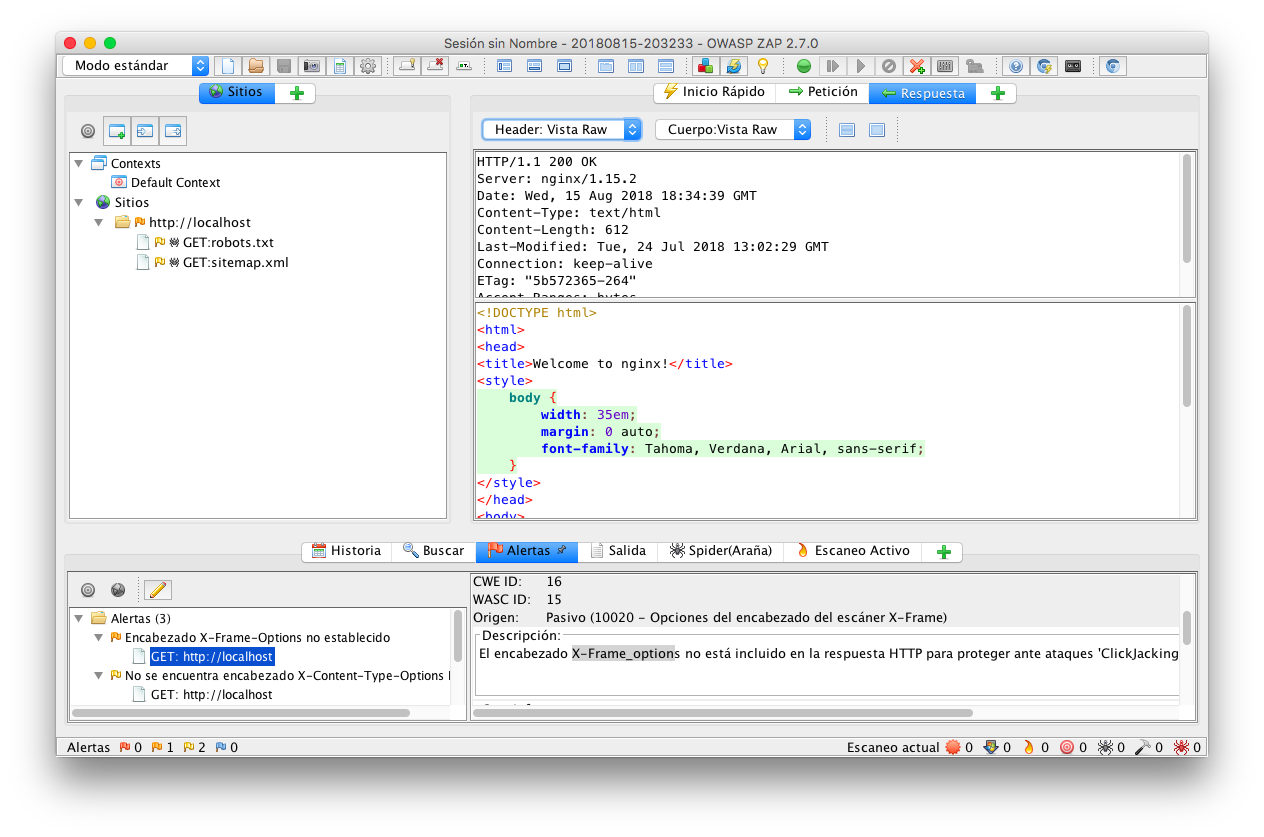
\includegraphics[width=1.0\textwidth]{../images/owasp-zap-main-window}
\caption{Ventana principal de OWASP ZAP}
\label{fig:owasp_zap}
\end{figure}


La última versión de NGINX (1.17.2) posee 739 directivas de configuración por lo que para simplificar nuestra tarea vamos a limitarnos a un conjunto mas pequeño de directivas (ver tabla \ref{table:apache_nginx_directives}).

\bigskip
En un primer momento pensamos en basarnos en las directivas \textbf{STIG}, pero estas directivas sólo están definidas para el servidor Apache. Por suerte al ser HTTP un estándar muchas de las directivas de Apache tienen su símil en NGINX por lo que hemos extraído un conjunto de las mas representativas y que además tuvieran su equivalente para el servidor NGINX. Las puntuaciones se basan en el sistema de puntuación CVSS de acuerdo con los resultados devueltos por ZAP con el código de prueba. También se han agregado algunas cabeceras identificativas como pueden ser la identificación del servidor (ver tabla \ref{table:ngingx_headers}) así como la directivas de compresión \texttt{gzip} para tener una mayor entropía.

\begin{table}[H]
\begin{tabular}{|l|l|l|l|}
\hline
Id & STIG ID & Configuración Apache  & Equivalente NGINX              \\ \hline
0  & V-13730 & MaxClients            & worker\_connections            \\ \hline
1  & V-13726 & KeepAliveTimeout      & keepalive\_timeout             \\ \hline
2  & V-13732 & FollowSymLinks        & disable\_symlinks              \\ \hline
3  & V-13735 & Indexes               & autoindex                      \\ \hline
4  & V-13724 & Timeout               & send\_timeout                  \\ \hline
5  & V-13738 & LimitRequestFieldsize & large\_client\_header\_buffers \\ \hline
6  & V-13736 & LimitRequestBody      & client\_max\_body\_size        \\ \hline
7  & V-6724  & ServerTokens          & server\_tokens                 \\ \hline
8  &         &                       & gzip                           \\ \hline
\end{tabular}
\label{table:apache_nginx_directives}
\caption{Lista de directivas NGINX utilizadas}
\end{table}

\begin{table}[H]
\begin{tabular}{|l|l|}
\hline
Id & Cabecera                       \\ \hline
9  & X-Frame-Options                \\ \hline
10  & X-Powered-By                   \\ \hline
11 & X-Content-Type-Options         \\ \hline
12 & Server                         \\ \hline
\end{tabular}
\label{table:ngingx_headers}
\caption{Lista de cabeceras HTTP utilizadas}
\end{table}

